\chapter{Generator}

\section{Storage of source data}

The generator of spatio-temporal and textual data uses real point of interests on the map as a source of data. These data where extracted from the online 
travel service TripAdvisor, using an already implemented crawler \cite{25}. These points of interest are identified on the map by their geographical coordinates, as 
well as their address. Also, they come with ratings and reviews by real TripAdvisor users. The number of such available points is 136409, as they were extracted by 
a 13GB response json file from the crawler. The points where stored in PostgreSQL. The database schema used, contains two tables, one for the points of interest 
and one for the reviews and ratings of these points and is the following:

\begin{figure}[H]
  \centering
  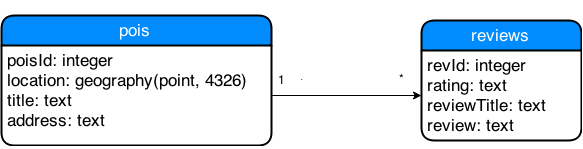
\includegraphics[width=0.7\textwidth]{figures/schema.png}
  \caption{Database schema for source data}
\end{figure}

More specifically, the table for the points of interest has the following attributes:

\begin{itemize}
 \item poisId: identifying number for the point of interest, primary key.
 \item location: geographical coordinates of the point. Usage of the geographic data type introduced by the extension PostGIS of PostgreSQL.
 \item title: the name of the point of interest.
 \item address: the address of the point on the map.
\end{itemize}

A point of interest can have many reviews, issued by different users, thus the two tables are associated by 1-to-many. The reviews table contains 
the following attributes:

\begin{itemize}
 \item revId: the identifying number of the point of interest that the review refers to, foreign key.
 \item rating: rating of the point in a scale of 1 to 5.
 \item reviewTitle: the title of the review.
 \item review: the text of the review.
\end{itemize}

After storing all points of interest into the database, we create an B-tree index to the attribute poisId of the table pois and to the attribute revId of the table reviews, 
as well. Additionally, we create a GiST index to the attibute location of the table pois. As location has a geographic data type, GiST will implement an 
improved R-tree index, as described in section 2.2.2. In this way, searching points of interest according to their location or identifying number, can be done 
fast and efficiently.

\section{Generator attributes}

The following class diagram indicates the main attributes used in the description of the generator's design.

\begin{figure}[H]
  \centering
  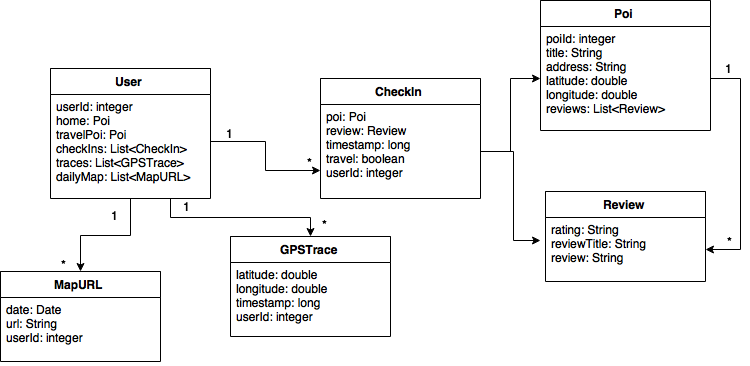
\includegraphics[width=0.9\textwidth]{figures/class_diagram.png}
  \caption{Class diagram of generator's attributes}
\end{figure}

\subsection{User}

The user produced by the generator has the following fields:

\begin{itemize}
 \item userId: user's identifier.
 \item home: user's home defined as Poi.
 \item travelPoi: the central location of the current trip, defined as Poi.
 \item checkIns: list of user's check-ins during the days for which the generator produced data.
 \item traces: list of GPS traces indicating the user's daily routes during the days for which the generator produced data.
 \item dailyMap: list of URLs to static maps images showing the daily user routes.
\end{itemize}

\subsection{Check-in}

A check-in to a point of interest (POI) has the following fields:

\begin{itemize}
 \item poi: the point of interest (POI) where the check-in was made.
 \item review: the review that the user made for the specfic POI on the check-in.
 \item timestamp: the time when the check-in was made, in representation of type long.
 \item travel: boolean value indicating whether the check-in was made during a user's trip.
 \item userId: the user's identifier.
\end{itemize}

\subsection{GPS trace}

A user's route consists of multiple GPS traces, which illustrate the path that the user followed. A GPS trace contains the following information:

\begin{itemize}
 \item (latitude, longitude): the geographical coordinates of the point on the map where the GPS trace was taken.
 \item timestamp: the time when the GPS trace was taken.
 \item userId: user's identifier whose route contains the specific GPS trace.
\end{itemize}

\subsection{Static route map - MapURL}

A user's daily route is depicted on a static map, using Google Static Maps API. The map shows the points of interest that the user visited using markers, 
and the exact path from one POI to another using blue continuous lines. The image of the map can be accessed through a respective URL.

\begin{itemize}
 \item url: the URL that directs to the image of the map.
 \item date: the date when the user walked the route showed on the map.
 \item userId: the identifier of the user who walked the specific route that date.
\end{itemize}

\subsection{Point of interest - Poi}

A point of interest has the following attributes:

\begin{itemize}
 \item poiId: point's identifier.
 \item title: point's name.
 \item address: point's address.
 \item (latitude, longitude): point's geographical coordinates.
 \item reviews: a list with the available reviews for the specific point.
\end{itemize}

\subsection{Review}

A review to a point of interest has the following fields:

\begin{itemize}
 \item rating: rating of the POI in scale 1 to 5.
 \item reviewTitle: the title of the review.
 \item review: the text of the review.
\end{itemize}

\section{Input parameters}

The generator takes as input the next parameters: 

\begin{itemize}
 \item userIdStart: identifier of the first user for whom the generator will create daily routes.
 \item userIdEnd: Respectively, the identifier of the last user created.
 \item chkNumMean: The mean of the number of daily check-ins to points of interest, which will follow a normal distribution.
 \item chkNumStDev: The standard deviation of the normal distribution that the number of daily check-ins follow.
 \item chkDurMean: The mean of the duration that each visit will last, which will follow a normal distribution.
 \item chkDurStDev: The standard deviation of the normal distribuition of the duration of user's visits.
 \item dist: The maximum distance in meters in which a user can walk from one point of interest to the next one.
 \item maxDist: The maximum distance in meters from a user's home, in which a user can walk every day.
 \item startTime: The time when the first check-in of the day will occur.
 \item endTime: The time when the last check-in of the day will occur.
 \item startDate: The first day starting from which the generator will create daily routes.
 \item endDate: Respectively, the last day that the generator will create daily routes.
 \item outCheckIns: The output file storing the daily check-ins of all users created.
 \item outTraces: The output files storing the GPS traces of the daily routes of all users created.
 \item outMaps: The output file storing the URLs for the daily maps depicting the daily routes of all users created.
\end{itemize}

\section{Generator's implementation definitions}

The generator's main function is to create user's daily routes, which will contain information simulating real social media data. These daily routes 
consist of visits (check-ins) to points of interest and paths that the user followed from one point to the next one. The generator takes as input the 
values of the corresponding parameters and based on the stored source data, creates daily routes for (userIdEnd - userIdStart + 1) users between 
the start and end dates. The decisions that the generator makes, such as which and how many points the user will visit a specific day, or the duration 
of each visit, are made using random factors. In this way, the produced data can be as realistic as possible. The generator stores the created data in three files, 
one for all the user check-ins (outCheckIns), one for the all the GPS traces (outTraces) and one for the all the daily maps (outMaps).

Briefly, the daily routes that the generator produces are designed in such a way that allows each user to visit places by walking from one point to the other. 
Each day, the user leaves his home and visits certain places that are in walking distance. The number of visits per day is decided in a random way. Moreover, 
the user stays for a couple of hours, also defined in a random way, at a point of interest and leaves a rating and review for that specific POI. Moving on, he walks 
to the next point, following the path that Google Directions API provides, and checks in to the next place. The generator enables a user to travel, following the 
same daily route strategy in the location of his trip.


\subsection{Home}

The location of a user's home is the center around which he walks every day. The points of interest that a user visits are selected in a random way, thus there can 
exist routes that don't make sense. For example, a user can walk one day in Greece, the next day in France and the other day again back in Greece. This is the reason 
why the location of a user's home is specified, so that a user can walk in a sensible distance from his home every day. More specifically, a user can walk in a range 
of maxDist meters from his home, as those are defined by the according input parameter. In the implementation of the generator, the home of a user is defined as 
the point where his first ever visit is made on startDate. The choice of this point is done using a generator of random numbers which follow a uniform distribution. 
The range of the distribution are the total number of source POIs stored in PostgreSQL.

\subsection{Trip}

A user created by the generator is capable to travel, so as to be able to visit places that are further than maxDist meters from his home. In this way, 
routes one day in Greece and the next one in France make sense. However, a central point around which the user will walk during his trip has to be defined. 
In the implementation of the generator, this point is chosen to be the first ever point that the user visits during the current trip. 
The choice of that point is done using a generator of random number that follow a uniform distribution. The range of the distribution is the number 
of available source POIs.

As far as the duration of each trip is concerned, each user can travel for a time interval that equals the 10\% of the total time interval for which the generator 
produces daily routes. The days of the time interval can be spread out to multiple trips. The duration of each trip is defined using a generator of random numbers 
which follow a normal distribution. The mean of this distribution is declared to be 5 and the standard deviation is 2. In this way, according to the 
3-sigma empirical rule for the normal distribution, 95\% of the random trip durations will be between 1 and 9 days, which is reasonable for short and long trips. 
To sum up, if the user is about to travel the next days, the duration of the trip is defined in a random way and if the duration of the trip doesn't exceed the 
available travel days, the prospective trip begins. If the duration of the trip exceeds the available days, then the trip is calculated to last for the 
available days.

Finally, the decision whether the user will begin a trip or not is made in a random way, using a generator of random numbers that follow the Bernoulli distribution. 
Thus, the generator decides every day whether or not to start a trip for the current user. This decision ressembles a fair coin toss. Therefore, 
if the generator decides to start a trip for the current user, then it decides, in a random way as well, the duration and the location of the trip. Each 
daily route during the trip has to be in maxDist range from the trip's central location.

\subsection{Check-in POI}

The number of daily check-ins is defined using a generator of random numbers that follow a normal distribution with a mean value determined by the input parameter 
chkNumMean and standard deviation determined by the input parameter chkNumStDev. Therefore, every day the generator picks a different number of daily check-ins, which 
according to the 3-sigma empirical rule for the normal distribution, will most probably be around the mean value.

The locations of check-ins are determined in a random way by the generator. More specifically, the choice of the point of interest, where the first check-in of the day 
will take place, is made using a generator of random number whio follow a uniform distribution. The range of this distribution is the number of available POIs 
who are located in maxDist range from the user's home. In this way, the generator will pick a random POI between those who are in walking distance from the user's home. 
If the user travels, then the generator will choose a random POI between those who are in maxDist range for the trip's central location. In order to find those 
points and select them from the PostgreSQL database, the function ST\_DWithin function is used, which is available through the PostGIS extension. 
This function returns true for the points which are in the desired distance from the user's home, calculating the distance using the geographical coordinates of the points. 
The search of these points in the PostgreSQL table is donw efficiently, due to the GiST index.
The generator will assemble all the points that are in the desired range, and choose a random one as the first point that the user visits in the current day. 

Using the same strategy, the generator chooses all next points of interest that the user will visit the specific day. However, the next points visited should be in 
a smaller distance from the first POI visited. This distance is defined by the input parameter dist. Also, a user is not allowed to visit the same place twice 
during the day, so every next check-in should be in a POI not visited that specific day.

\subsection{Check-in review}

The generator assigns a rating and review to every user's check-in. More specifically, every source point of interest as it is stored in PostgreSQL database, 
contains certain reviews for the specific point. The generator chooses randomly a review amongst the available for the POI, using a generator of random 
numbers that follow a uniform distribution. The range of the distribution is the number of available reviews for the specific POI.

\subsection{Path between check-ins}

The generator issues an http request to Google Directions API, in order to obtain information about the path that a user will follow in order to walk from one point 
of interest to the next one. Since the source data contain the geographical coordinates of every point of interest, the generator has access to the latitude and 
longitude of every available point. Thus, he sets as value of the origin parameter to the http request the geographical coordinates of the current point where 
the user checked in and as destination the coordinates of the next point of interest that the user will visit, as it was selected in a random way. Also, he 
specifies the paramater mode into walking, because the user walks from one POI to the next one. Finally, the response file of the request will be in json file format. 
For example, a request to Google Directions API can be the following:
\begin{center}
 http://maps.googleapis.com/maps/api/directions/json?origin=37.976159, 23.776274\&destination=37.978180, 23.768957\&mode=walking
\end{center}

The json response file contains information about the path on the map, that the user will have to follow in order to get to his destination, as well as the duration of 
his walk to the destination. We extract from the json file, the field polyline from each step of the route. The polyline holds an encoded representation of the step's 
path. We decode each step's polyline using the reverse Encoded Polyline Algorithm Format, as it was described in section 2.4.2. In this way, we have access 
to a list of geographical coordinates indicating all the points on the map, that the user will walk through from the origin to the destination. These points 
will be stored as GPS traces, representating the user's route. For each path, the starting and ending points, which are the points of interest, will also be stored 
as GPS traces.

\subsection{Timestamp}

As far as time is concerned, the generator defines that the first check-in of the day will happen at the time defined by the input parameter startTime. 
The duration of the visit to a point of interest is set 
using a generator of random numbers that follow a normal distribution. The mean value of the distribution is defined by the chkDurMean input parameter, and 
the standard deviation by the chkDurStDev parameter. The time when the next check-in will occur is set to be the time when the previous one happened, plus 
the duration of the previous visit and the duration of the walk from the previous point to the next one. The duration of the walk, is extracted from 
the field duration of the Google Directions json response file. If the time that the next check-in will happen exceeds the time defined by the input parameter 
endTime, then the next check-in won't occur, and the check-ins end at that time for that specific day. Each check-in is timestamped 
using the Unix Time Stamp, which is a long integer representation of the date and specific time (UTC timezone) of the event.

Concerning the timestamp of the GPS traces, they are calculated through the json response file. The duration of the route from the origin to the destination is 
splitted up by the number of points decoded from the polyline. Therefore, the timestamp of the first GPS trace of the path is set to be the time the visit 
at the origin ended plus the fraction of the divided time needed to get to that point on the map.

\subsection{Static map}

The generator uses a static map in order to depict the user's daily route, by issuing an http request to the Google Static Maps API. 
The points where a user checked in during the day are distinctly visible on the map with markers. These markers are also named using capital 
letters of the alphabet in order to show the order that the user visited them. The generator uses the stored polylines, as they were extracted by the json 
response file, in order to define the path that the map will indicate using a blue continuous line. The image of the map is accessible through the URL that 
forms the http request to the API. The generator stores the URLs created at the corresponding output file (outMaps), so that the image of the map can 
be accessible by the users of the generator.

For example, a request to Google Static Maps API, 
as it is created by the generator, can be the following:
\begin{center}
\url{https://maps.googleapis.com/maps/api/staticmap?&size=1000x1000&markers=label:A|44.7698,-69.7215&markers=label:B|44.7651,-69.7189&markers=label:C|44.7639,-69.7196&markers=label:D|44.7656,-69.717&path=color:blue|enc:gbgpGjnphL@FZKtE_BxEeB`Bk@z@[bA]tBo@HG~Ai@JMFG?A@A?A@C?C?E?C?EAE?I??M_@??L^??Tj@Vl@LNDFDDFDDDB@DBD@HBLBRBB?H@JAF?DAFAHCFCDCBCDEDGNU??OTEFEDCBEBGBIBG@E@G?K@IAC?SCMCICEAECCAEEGEEEEGMO??Wm@Uk@cAyCs@_C??bA_A}
\end{center}
The map that corresponds to the above URL is:

\begin{figure}[H]
  \centering
  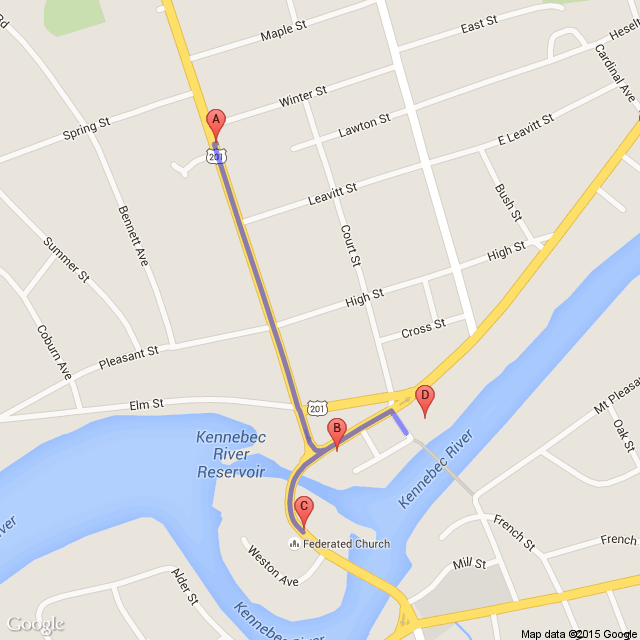
\includegraphics[width=0.7\textwidth]{figures/staticmap.png}
  \caption{Example of static map image}
\end{figure}









